%%%%%%%%%%%%%%%%%%%%%%%%%%%%%%%%%%%%%%%%%
% a0poster Landscape Poster
% LaTeX Template
% Version 1.0 (22/06/13)
%
% The a0poster class was created by:
% Gerlinde Kettl and Matthias Weiser (tex@kettl.de)
% 
% This template has been downloaded from:
% http://www.LaTeXTemplates.com
%
% License:
% CC BY-NC-SA 3.0 (http://creativecommons.org/licenses/by-nc-sa/3.0/)
%
%%%%%%%%%%%%%%%%%%%%%%%%%%%%%%%%%%%%%%%%%

%----------------------------------------------------------------------------------------
%	PACKAGES AND OTHER DOCUMENT CONFIGURATIONS
%----------------------------------------------------------------------------------------

\documentclass[a0,landscape]{a0poster}

\usepackage{multicol} % This is so we can have multiple columns of text side-by-side
\columnsep=100pt % This is the amount of white space between the columns in the poster
\columnseprule=3pt % This is the thickness of the black line between the columns in the poster

\usepackage[svgnames]{xcolor} % Specify colors by their 'svgnames', for a full list of all colors available see here: http://www.latextemplates.com/svgnames-colors

\usepackage{pgfpages}
\pgfpagesdeclarelayout{resize and center}
{
  \def\pgfpageoptionborder{0pt}
}
{
  \pgfpagesphysicalpageoptions
  {%
    logical pages=1,%
    physical height=\pgfpageoptionheight,%
    physical width=\pgfpageoptionwidth%
  }
  \pgfpageslogicalpageoptions{1}
  {%
    resized width=\pgfphysicalwidth,%
    resized height=\pgfphysicalheight,%
    border shrink=\pgfpageoptionborder,%
    center=\pgfpoint{.5215\pgfphysicalwidth}{.47\pgfphysicalheight}%
  }%
}
\pgfpagesuselayout{resize and center}[a2paper,landscape]

\usepackage{times} % Use the times font
%\usepackage{palatino} % Uncomment to use the Palatino font

\usepackage{graphicx} % Required for including images
\graphicspath{{figures/}} % Location of the graphics files
\usepackage{booktabs} % Top and bottom rules for table
\usepackage[font=small,labelfont=bf]{caption} % Required for specifying captions to tables and figures
\usepackage{amsfonts, amsmath, amsthm, amssymb} % For math fonts, symbols and environments
\usepackage{wrapfig} % Allows wrapping text around tables and figures

\begin{document}

%----------------------------------------------------------------------------------------
%	POSTER HEADER 
%----------------------------------------------------------------------------------------

% The header is divided into three boxes:
% The first is 55% wide and houses the title, subtitle, names and university/organization
% The second is 25% wide and houses contact information
% The third is 19% wide and houses a logo for your university/organization or a photo of you
% The widths of these boxes can be easily edited to accommodate your content as you see fit

\begin{minipage}[b]{0.55\linewidth}
\veryHuge \color{DarkOrange} \textbf{Location Sensitive Social Notifier} \color{Black}\\ % Title
\Huge\textit{Location based, messaging platform for Android smartphones}\\[1cm] % Subtitle
\huge \textbf{Thomas Mark Rosier}\\ % Author(s)
\huge Aberystwyth University, Computer Science Department\\ % University/organization
\end{minipage}
%
\begin{minipage}[b]{0.25\linewidth}
\color{DarkSlateGray}\Large \textbf{Contact Information:}\\
Department of Computer Science\\
Llandinam Building\\
Aberystwyth University\\
Aberystwyth\\
Ceredigion\\
SY23 3DB\\ 
Email: \texttt{thr2@aber.ac.uk}\\ % Email address
\end{minipage}
%
\begin{minipage}[b]{0.19\linewidth}
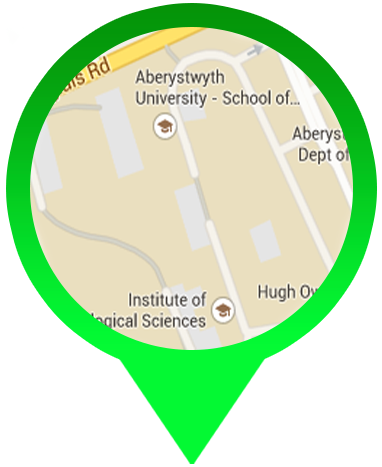
\includegraphics[width=12cm]{logo.png} % Logo or a photo of you, adjust its dimensions here
\end{minipage}

\vspace{1cm} % A bit of extra whitespace between the header and poster content

%----------------------------------------------------------------------------------------

\begin{multicols}{4} % This is how many columns your poster will be broken into, a poster with many figures may benefit from less columns whereas a text-heavy poster benefits from more

\section{Abstract}

\section{Introduction}

\section{Aims of the project}

\section{Progress so far}

\section{Technical details}

\section{Future development}

%----------------------------------------------------------------------------------------

\end{multicols}
\end{document}